\section{Usage of LLMs}
\label{sec:llm_usage}
Throughout the preparation of this manuscript, we used LLMs to assist with improving grammar, clarity, and wording in parts of this work. The use of LLMs was limited to language refinement, with all ideas, analyses, and conclusions solely developed by the authors.

\begin{figure*}[htbp]
    \centering
    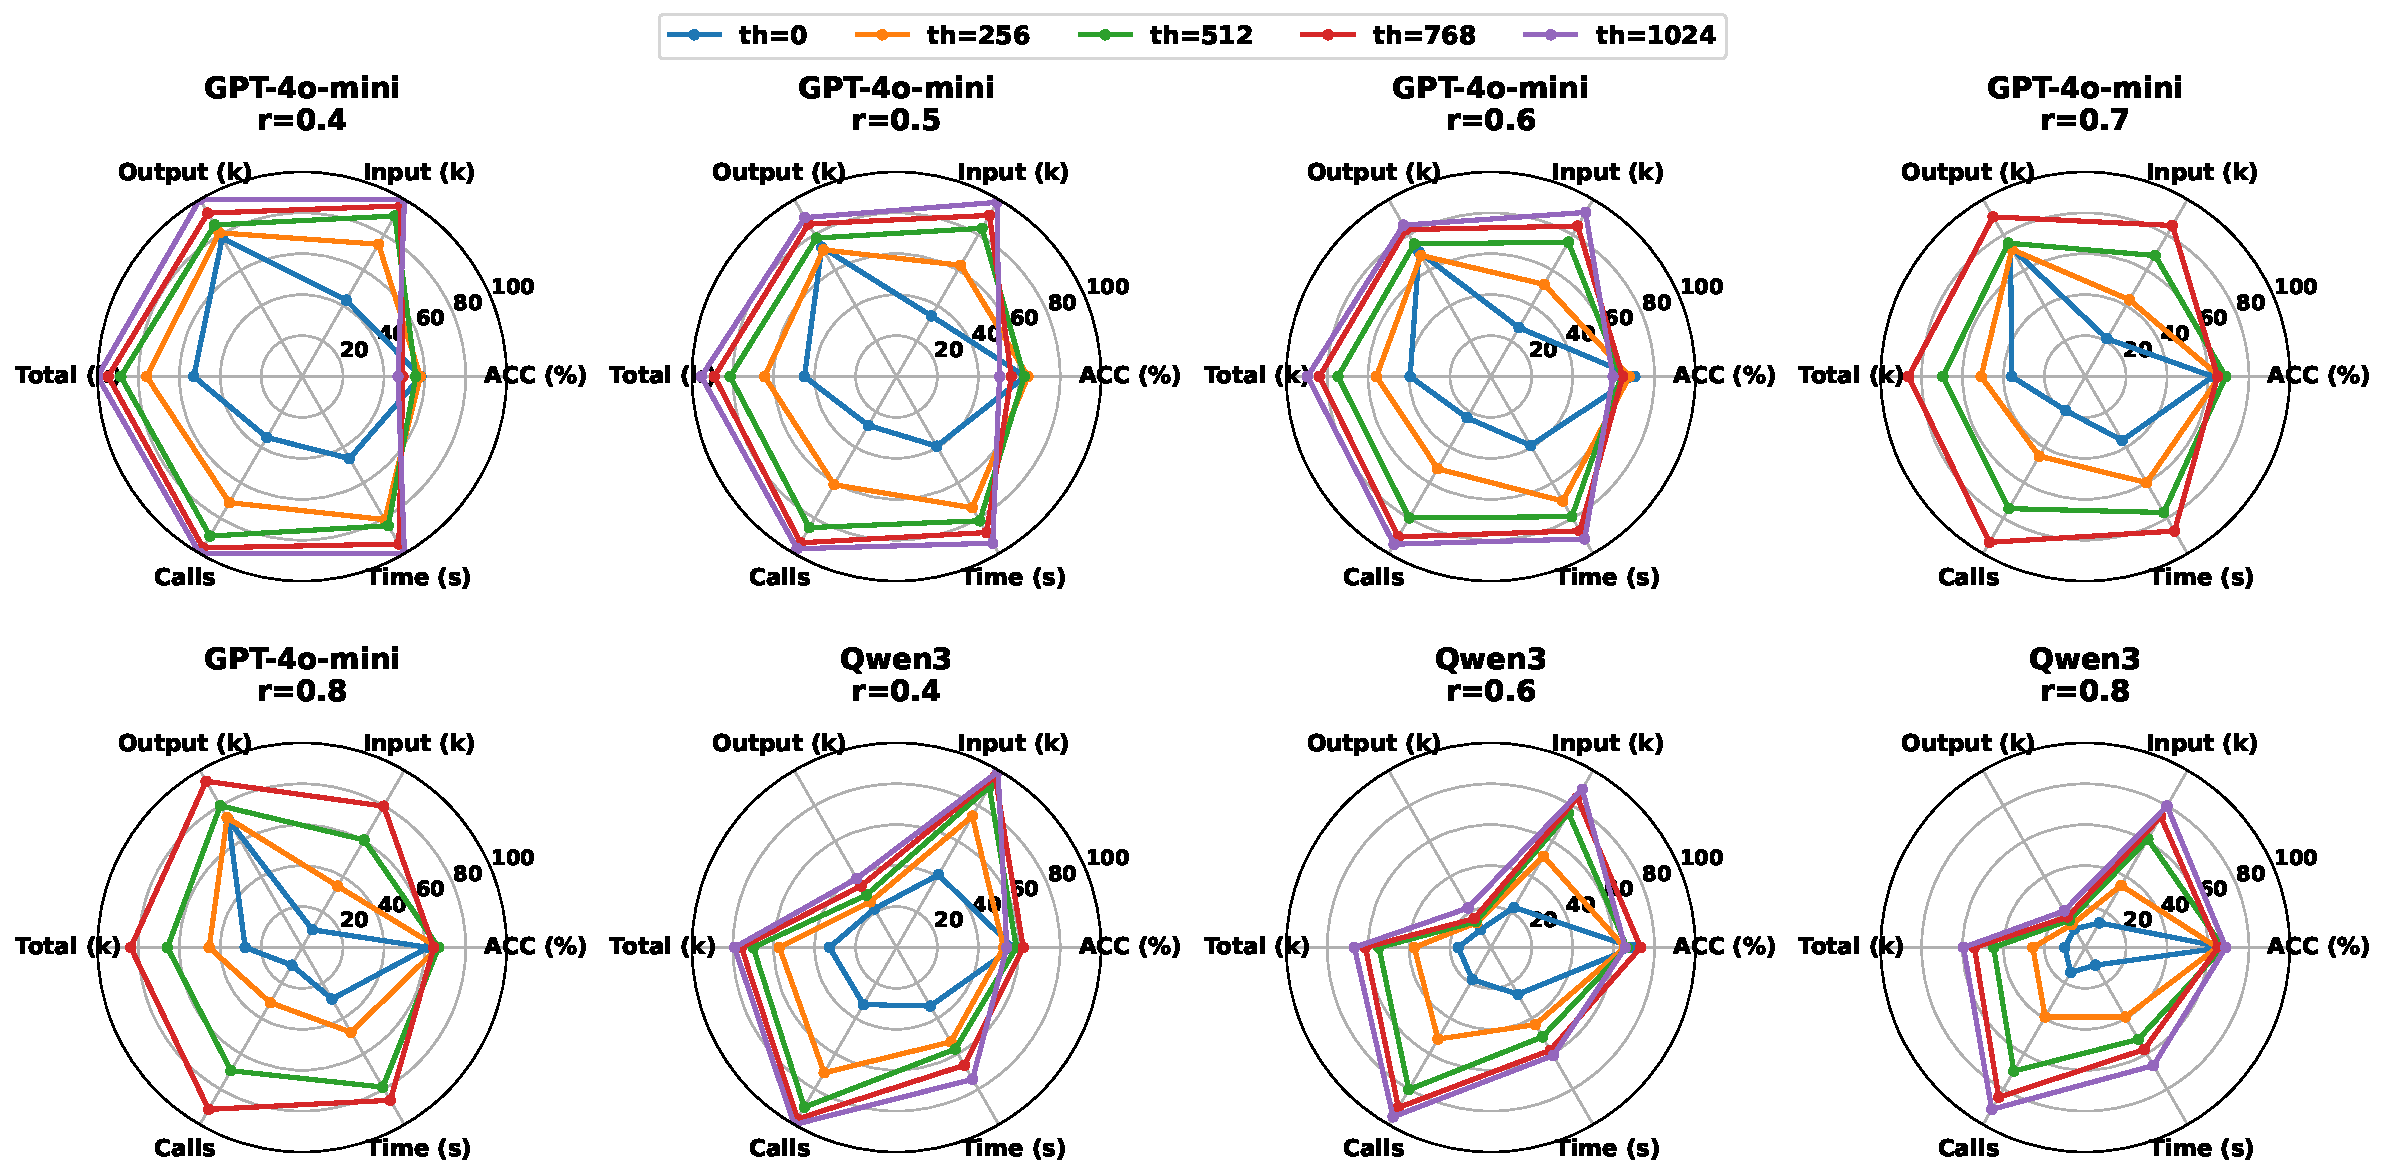
\includegraphics[width=1\textwidth]{figure/lightmem_radar.pdf}
    \caption{
Impact of the STM buffer threshold ($th$) on performance and efficiency across different compression ratios ($r$). 
Each radar chart represents a specific configuration of a model (GPT-4o-mini or Qwen3) and a fixed compression ratio. 
The axes measure six key metrics: Accuracy (ACC), token consumption (Input, Output, Total), API Calls, and Runtime. 
To facilitate comparison, all values are normalized for visualization on the chart. 
}
\label{fig:lightmem_radar}
\end{figure*}





\section{Methodology Details}
\label{appendix-setup}
\subsection{Topic Segmentation}
\label{appen_topic_seg}

In this part, we present the construction of the attention matrix, the underlying rationale for topic segmentation, and representative illustrative cases.
%The specific construction method of turn-level attention matrix
%这里写具体这个矩阵是怎么算的：turn-level、前后三个token去掉、一个turn-level的总注意力是由这个turn所有token的注意力的平均值 balabala

%%%%%%%%%%%%%
We extract only the user sentences from multi-turn dialogues, as they are generally more concise and the assistant’s responses necessarily remain consistent with the user’s theme within the same turn. Moreover, since the maximum input length of the LLMLingua-2 \cite{pan2024llmlingua} model is 512 tokens, the assistant’s often lengthy sentences cannot be effectively accommodated. Therefore, we sequentially store the user sentences into a buffer and segment them, ensuring that as many sentences as possible are preserved while staying within the token limit. As a practical trick, if a sentence becomes empty after compression, we retain its original uncompressed version; if the token length of a sentence still exceeds the maximum limit, we continue to compress it using the LLMLingua-2 model at a 0.5 compression rate until the token length falls below the threshold. To reduce the effect of attention sinks, we mask out the contributions of the first and last three tokens in each sequence and subsequently normalize the remaining attention values. Attention is derived from the higher layers of LLMLingua-2 (layers 8, 9, 10, and 11). For any two sentences, we first compute token-level pairwise attention and average across tokens to obtain the overall attention of one sentence to the target sentence; we then average across the selected layers to obtain a more robust inter-sentence attention score. For each current sentence, the attention scores directed toward all preceding sentences are normalized within the sentence, yielding the final attention matrix. Residual fragments that remain after segmentation are carried over to the beginning of the next buffer for further processing, and this procedure continues iteratively until the dialogue ends.

%%%%%%%%%%%%%%


%the detailed rationale for topic segmentation
%这个部分就是写具体怎么切割，某个位置出现了一个局部峰值点，就在这个位置切割（这里要写清楚峰值点的下标和分割点下标，数字上可能相差1）；然后要写一下我们为什么要在这个局部峰值点去切割，就是topic转变之后，注意力会怎么怎么变 balabala，这一块我之前口头和你解释过

%%%%%%%%%%%%%%
Based on the attention pattern, we focus on the sequence formed by each sentence’s attention scores relative to its immediately preceding sentence, which directly reflects the continuity of local semantics. Therefore, we take the attention scores from the outermost layer of the attention map. When the attention score at a given position is higher than both its preceding and following positions, it is regarded as a local peak. If a sentence is identified as a peak, we set a segmentation point immediately before this sentence, making the peak sentence the beginning of a new segment. The rationale is that the peak sentence exhibits consistently low attention to all earlier sentences overall and reflects a clear transition from an old topic to a new one, indicating that the identified sentence marks the initiation of a new topic.
%%%%%%%%%%%%%%

\begin{figure}[H]
    \centering
    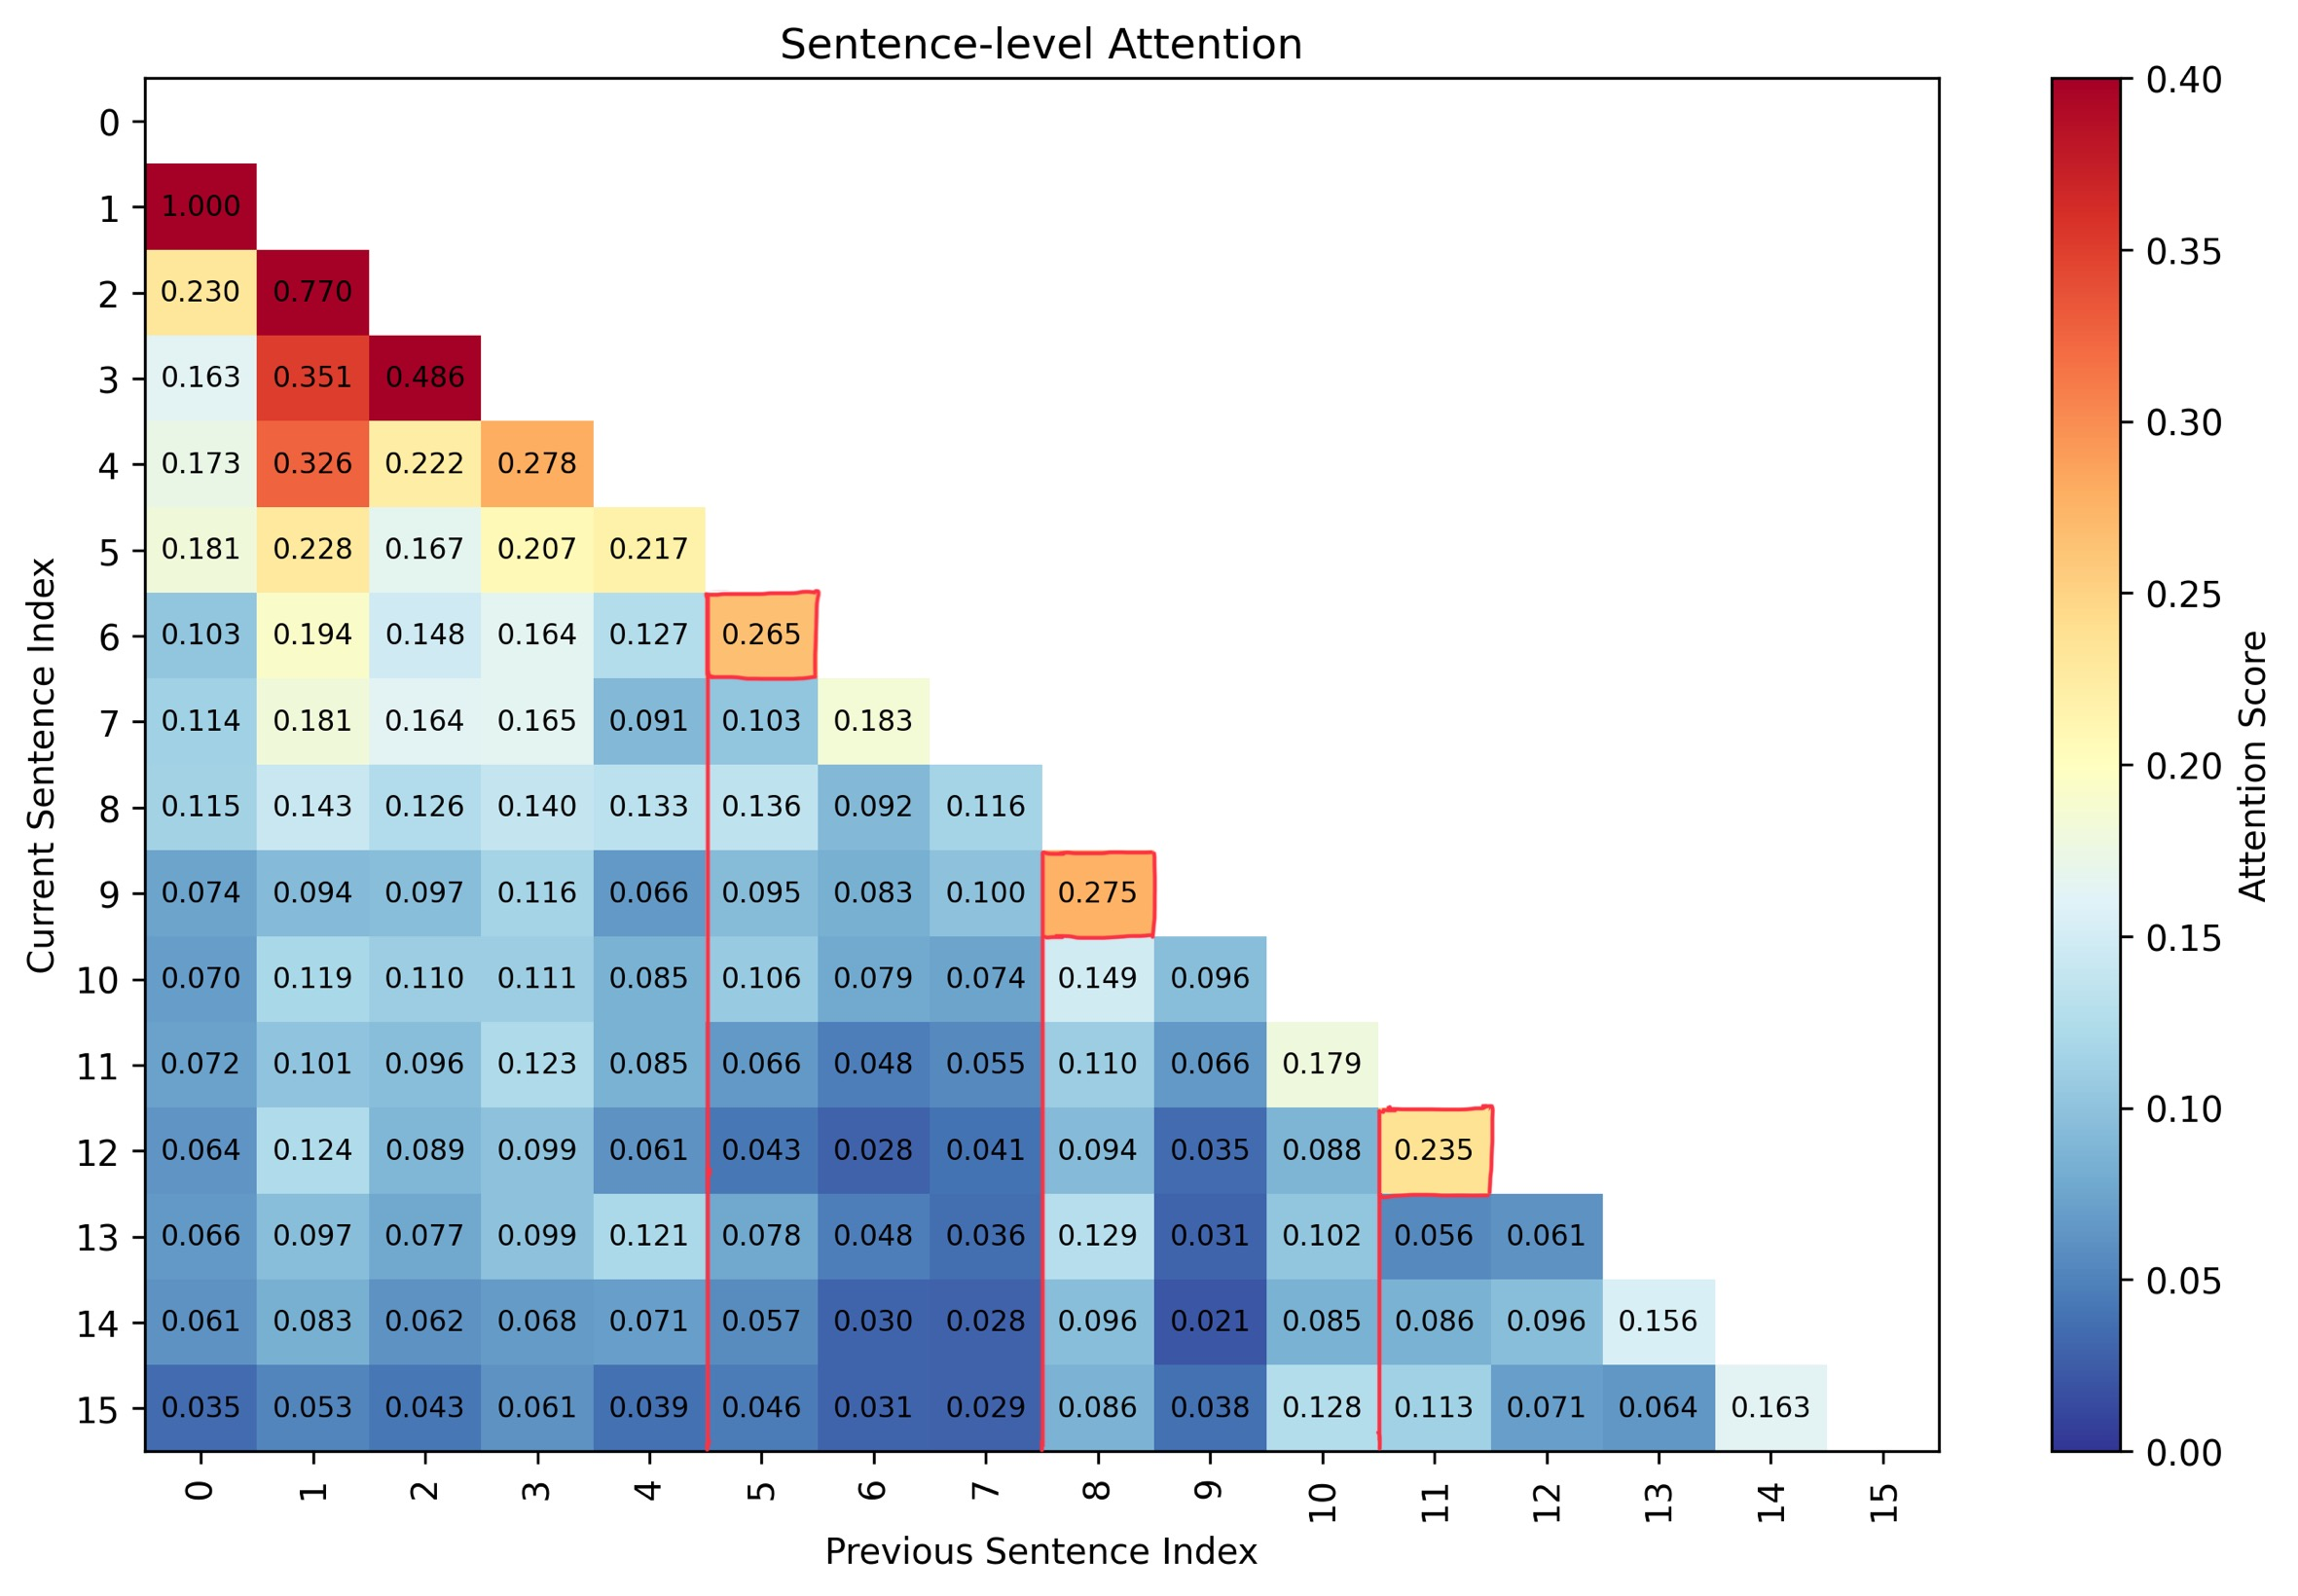
\includegraphics[width=0.48\textwidth]{figure/Attention_Matrix1.png}
    \hfill
    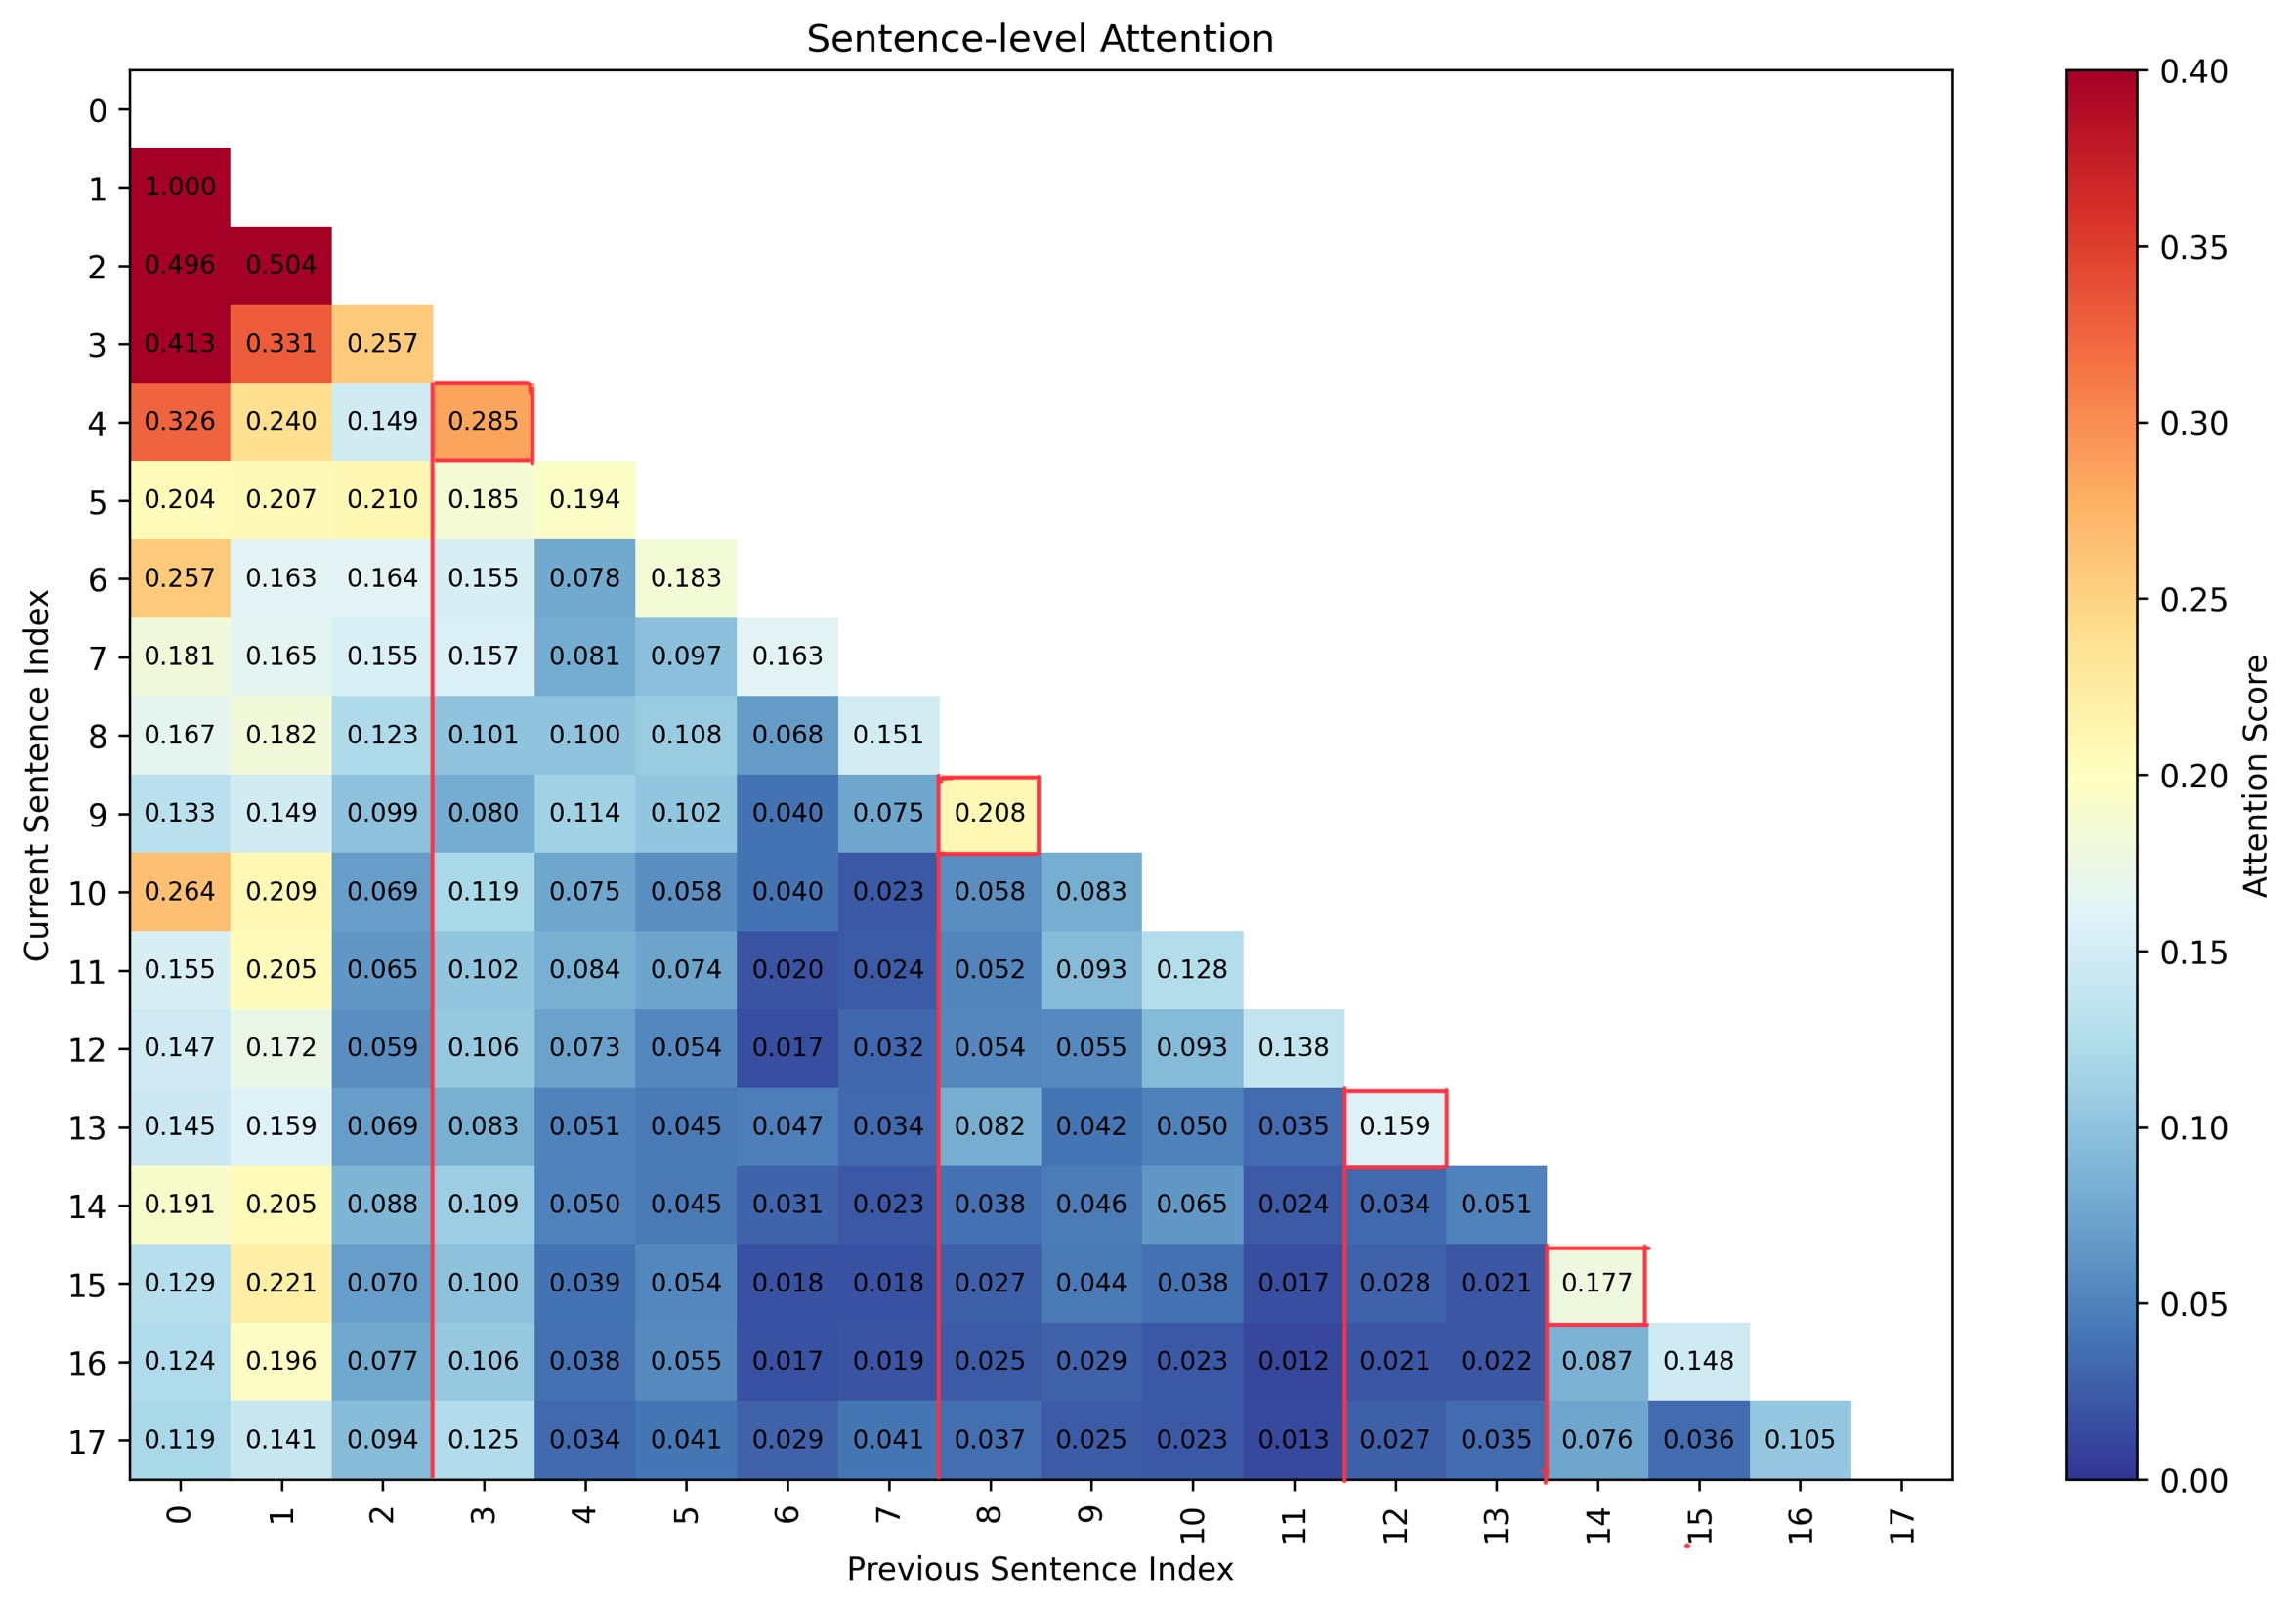
\includegraphics[width=0.48\textwidth]{figure/Attention_Matrix2.png}
    % \hfill
    % 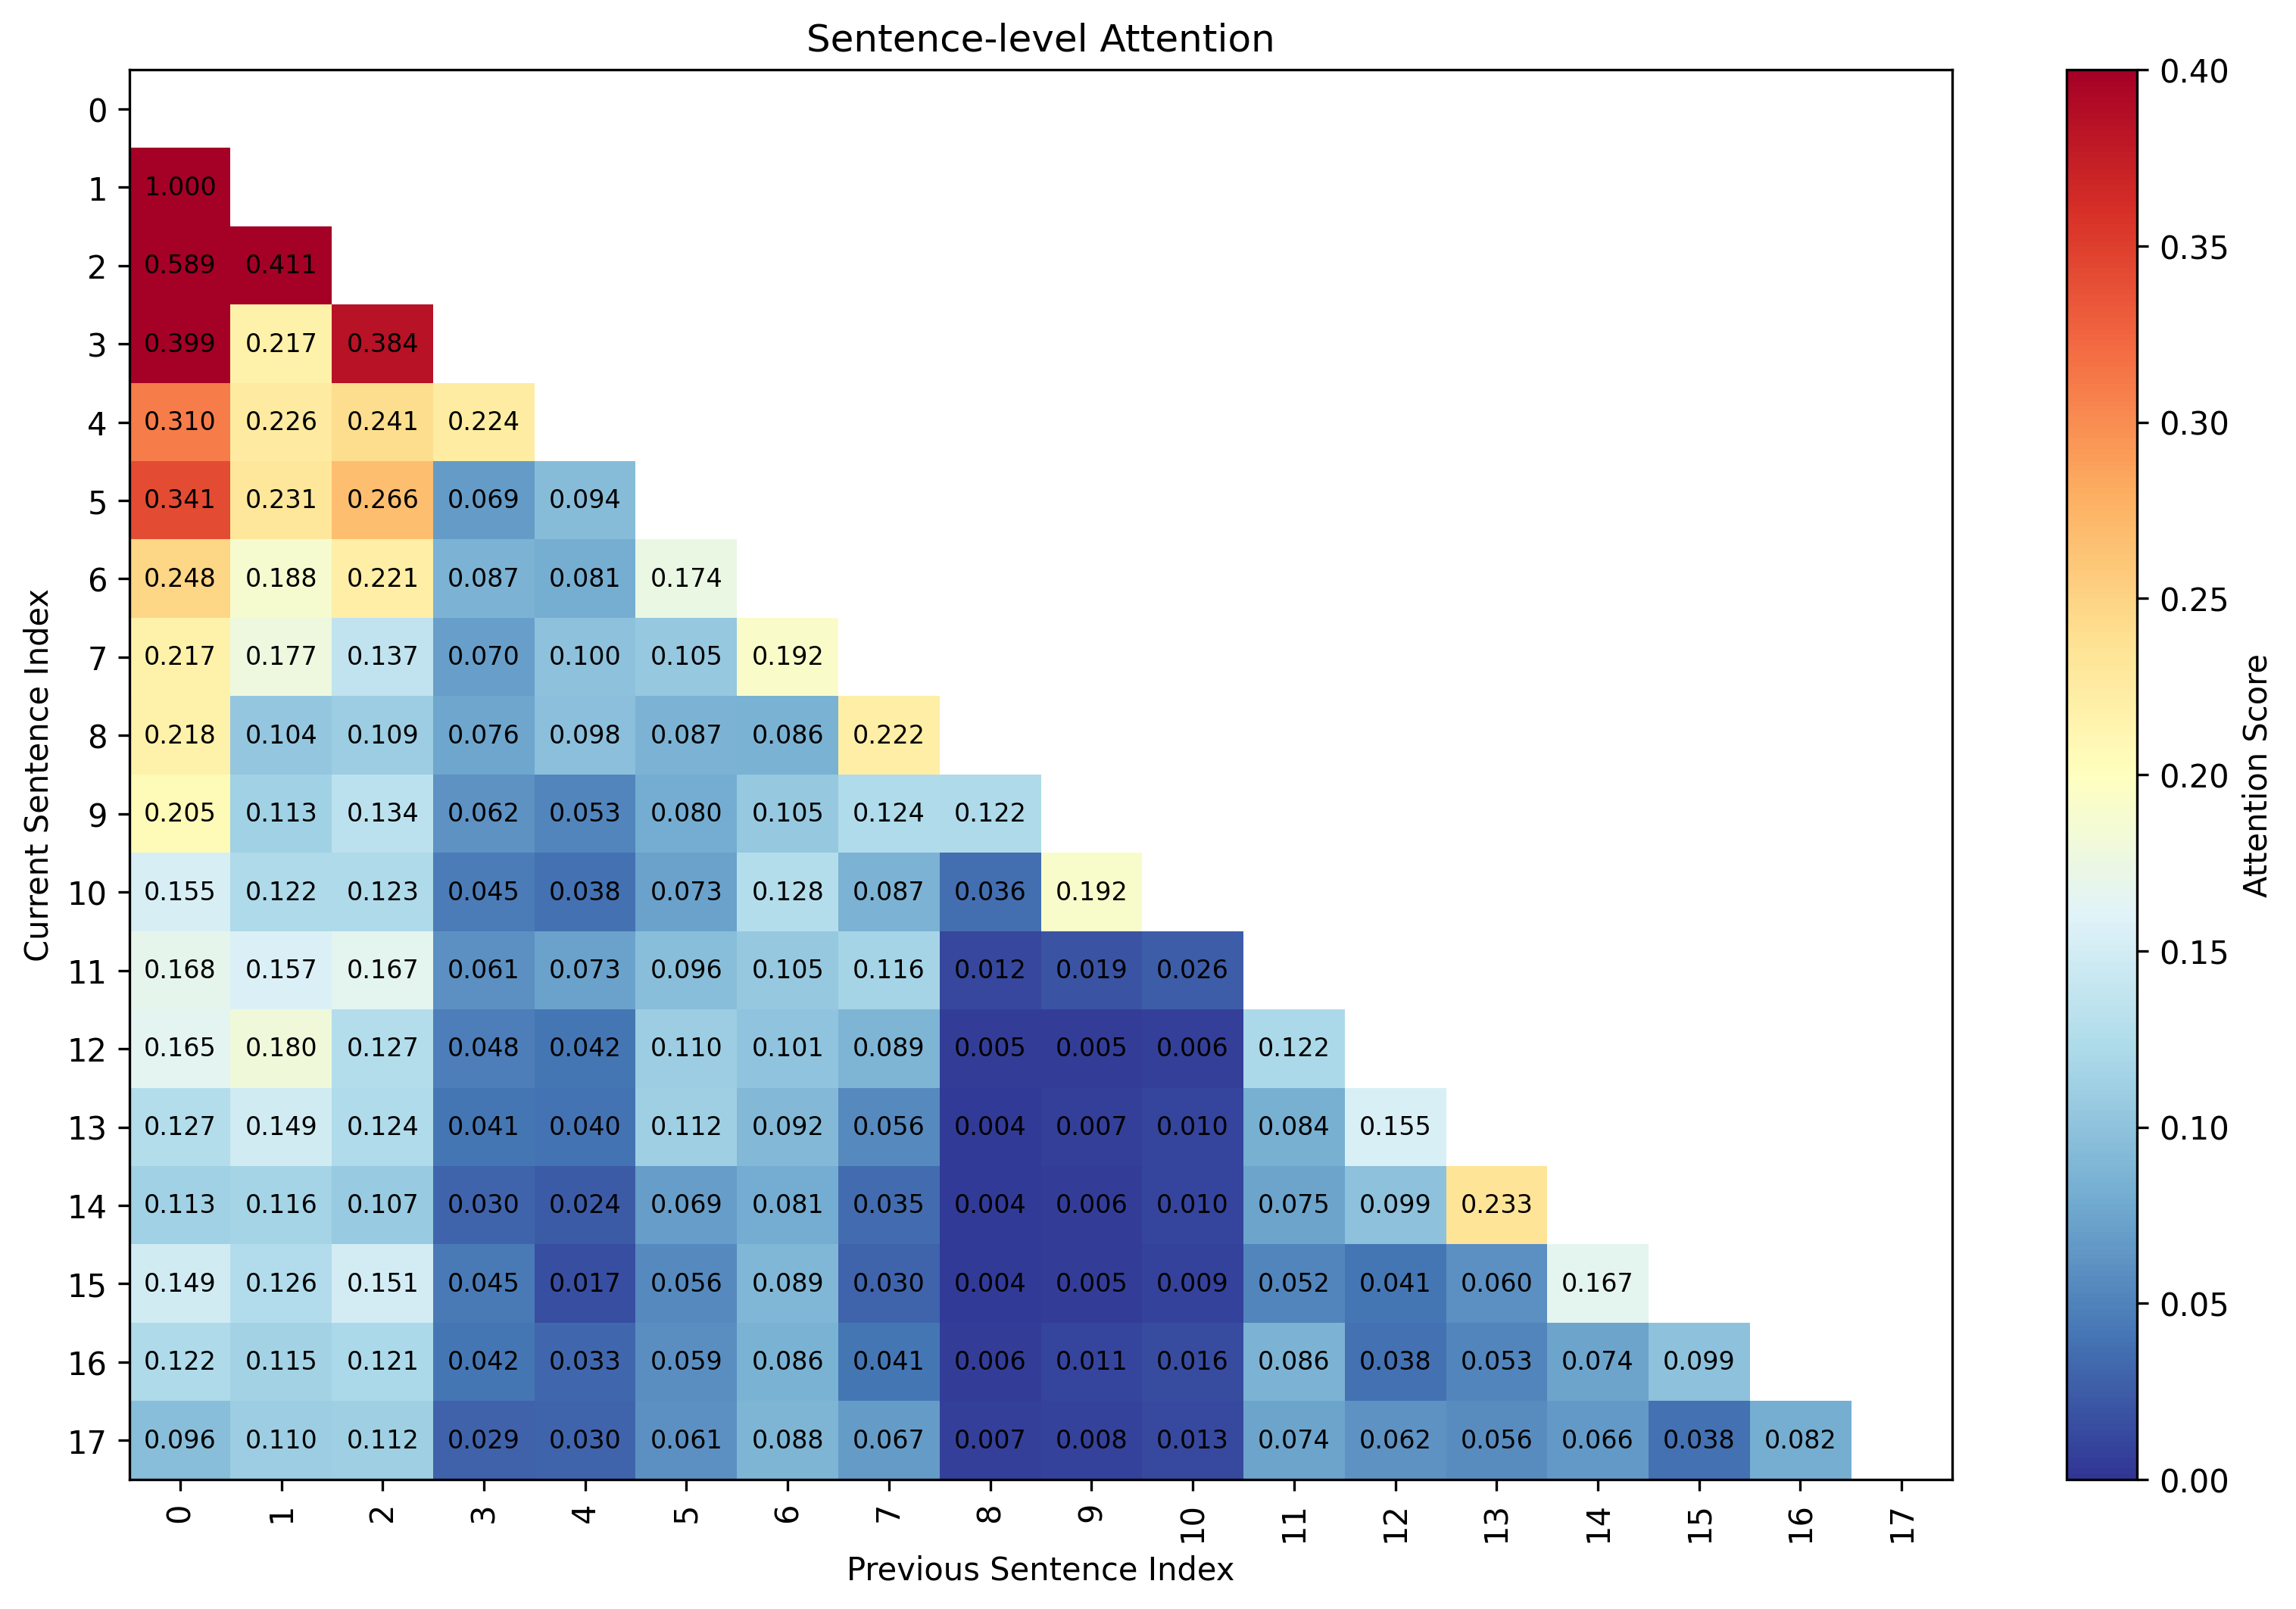
\includegraphics[width=0.32\textwidth]{figure/Attention_Matrix3.png}
    \caption{Example of Topic Segment Attention Matrix.}
    \label{fig:attention_matrix}
\end{figure}

%illustrative cases
%就是给个切割得准一点的case，贴一个注意力图，然后标注一下切割点，然后说明我们方法切割得很准

%%%%%%%%%%%%%%%
Figure \ref{fig:attention_matrix} illustrates three representative examples of reliable segmentation under 50\% compression rate. In the first attention map, local peaks in the adjacent-sentence attention sequence appear at positions 5, 8, and 11, where the actual segmentation boundaries lie between sentences 4–5 and 11–12. In the second attention map, peaks occur at positions 3, 8, 12, and 14, and the actual boundaries are located between sentences 7–8, 11–12, and 13–14. 
% In the third attention map, local peaks are observed at positions 7, 9, and 13, while the final segmentation boundaries fall between sentences 6–7, 8–9, and 14–15.
Overall, our method achieves close alignment with the majority of true boundaries while providing finer-grained segmentation. These examples demonstrate that our segmentation approach enables both fine-grained and reliable detection of topic boundaries, thereby validating its effectiveness. 
%%%%%%%%%%%%%%%

\subsection{Category-wise Accuracy}
As summarized in Table~\ref{tab:catwise_acc_by_model}, retrieval-augmented and memory-centric methods (e.g., \textit{A-MEM}, \textit{Mem0}, \textit{MemoryOS}) generally outperform \textit{Full Text} on categories that demand information integration or belief revision, such as \emph{Temporal}, \emph{Multi-Session}, and \emph{Knowledge-Update}.
In contrast, categories such as \emph{Single-User} and \emph{Single-Assistant}, lightweight retrieval like \textit{Naive RAG} is often competitive and can be the most reliable option, while \emph{Single-Preference} shows higher variance due to its smaller sample size. 

\begin{table*}[htbp]
\centering
\caption{\textbf{Category-wise Accuracy}. Accuracy (\%) by method across question types. Parentheses indicate category proportion and sample size. For GPT, LightMem is configured with parameters $r=0.7$ and $\text{th}=512$; for Qwen, LightMem is configured with $r=0.4$ and $\text{th}=768$.
}
\vspace{0.5ex}
\renewcommand{\arraystretch}{1.1}
\setlength{\tabcolsep}{3pt}
\small
\scalebox{0.95}{
\begin{threeparttable}
\begin{tabular}{@{}lcccccc@{}}
\toprule
\textbf{Method} &
\makecell{\textbf{Temporal}\\\makecell{\footnotesize ( $n{=}133$)}} &
\makecell{\textbf{Multi-Session}\\\makecell{\footnotesize ($n{=}133$)}} &
\makecell{\textbf{Knowledge-Update}\\\makecell{\footnotesize ($n{=}78$)}} &
\makecell{\textbf{Single-User}\\\makecell{\footnotesize ($n{=}70$)}} &
\makecell{\textbf{Single-Assistant}\\\makecell{\footnotesize ($n{=}56$)}} &
\makecell{\textbf{Single-Preference}\\\makecell{\footnotesize ($n{=}30$)}} \\
\midrule

% ===== GPT-4o-mini section =====
\rowcolor{gptbar}\multicolumn{7}{c}{\openailogo\ \textbf{GPT-4o-mini}}\\
\midrule
\rowcolor{gptgray} \textit{Full Text}    & 31.58 & 45.45 & 76.92 & 87.14 & 89.29 & 36.67 \\
\rowcolor{gptgray} \textit{Naive RAG}    & 39.85 & 48.48 & 67.95 & 90.00 & 98.21 & 53.33 \\
\rowcolor{gptgray} \textit{LangMem}      & 15.79 & 20.30 & 66.67 & 60.00 & 46.43 & 60.00 \\
\rowcolor{gptgray} \textit{A-MEM}        & 47.36 & 48.87 & 64.11 & 92.86 & 96.43 & 46.67 \\
\rowcolor{gptgray} \textit{MemoryOS}     & 32.33 & 31.06 & 48.72 & 80.00 & 64.29 & 30.00 \\
\rowcolor{gptgray} \textit{Mem0}         & 40.15 & 46.21 & 70.12 & 81.43 & 41.07 & 60.00 \\
\rowcolor{gptgray} \textit{LightMem}     & 67.18 & 71.74 & 83.12 & 87.14 & 32.14 & 68.18 \\

\addlinespace[0.4ex]
\midrule

% ===== Qwen section =====
\rowcolor{qwenbar}\multicolumn{7}{c}{\qwenlogo\ \textbf{Qwen3-30B-A3B-Instruct-2507}}\\
\midrule
\rowcolor{qwenlav} \textit{Full Text}    & 33.08 & 35.61 & 76.92 & 82.86 & 87.50 & 50.00 \\
\rowcolor{qwenlav} \textit{Naive RAG}    & 36.84 & 47.73 & 65.38 & 91.43 & 98.21 & 70.00 \\
\rowcolor{qwenlav} \textit{LangMem}      & 37.60 & 38.35 & 67.95 & 78.57 & 42.86 & 70.00 \\
\rowcolor{qwenlav} \textit{A-MEM}        & 51.88 & 51.12 & 76.93 & 90.00 & 96.43 & 40.00 \\
\rowcolor{qwenlav} \textit{MemoryOS}     & 28.57 & 36.84 & 61.54 & 72.86 & 92.86 & 33.33 \\
\rowcolor{qwenlav} \textit{Mem0}         & 41.94 & 28.13 & 28.57 & 55.32 & 26.09 & 81.82 \\
\rowcolor{qwenlav} \textit{LightMem}         & 54.20 & 51.91 & 66.67 & 80.00 & 31.25 & 80.00 \\
\bottomrule
\end{tabular}
\end{threeparttable}
}
\label{tab:catwise_acc_by_model}
\end{table*}

% LightMem补充后完善
% Single-Preference的方差可以稍微分析一下


% \subsection{Cost of Retrieval-Augmented Responses}
% \begin{table}[htbp]
\centering
\caption{\textbf{Cost of Retrieval-Augmented Responses}. Average end-to-end time (seconds) for \emph{Search + Answer} per query. \textit{Full Text} has no retrieval, so the time reflects answer latency only.}
\label{tab:rag_cost_time}
\renewcommand{\arraystretch}{1.05}
\setlength{\tabcolsep}{5pt}
\scriptsize
\begin{tabular}{@{}lcc@{}}
\toprule
\multirow{2}{*}{\textbf{Method}} & \multicolumn{2}{c}{\textbf{Avg Time (s)}} \\
\cmidrule(lr){2-3}
& \cellcolor{gptgray}\textbf{\openailogo GPT-4o-mini} & \cellcolor{qwenlav}\textbf{\qwenlogo Qwen3-30B-A3B-Instruct-2507} \\
\midrule
\textit{Full Text} & \cellcolor{gptgray} 11.50 & \cellcolor{qwenlav}-- \\
\textit{Naive RAG} & \cellcolor{gptgray}6.57 & \cellcolor{qwenlav} 5.50 \\
\textit{LangMem} & \cellcolor{gptgray}-- & \cellcolor{qwenlav}-- \\
\textit{A-MEM} & \cellcolor{gptgray}-- & \cellcolor{qwenlav}-- \\
\textit{MemoryOS} & \cellcolor{gptgray} 2.15 & \cellcolor{qwenlav} 1.64 \\
\textit{Mem0} & \cellcolor{gptgray} 8.77 & \cellcolor{qwenlav} 7.80 \\
\textit{LightMem} & \cellcolor{gptgray}-- & \cellcolor{qwenlav}-- \\
\bottomrule
\end{tabular}
\end{table}

\subsection{Detailed Parameter Analysis}
\label{lightmem_results}
As Table~\ref{tab:lightmem_comparison} shows, we report the numerical results of the effects of LightMem parameters (compression ratio $r$ and STM threshold $th$).


\begin{table*}[ht]
\centering
\caption{The impact of \textbf{LightMem} compression ratio $r$ and STM buffer threshold $th$ is reported here. Due to space limitations, we only present a subset of representative results of the online soft update results, with more results provided in the Figure~\ref{tab:lightmem_comparison}.}
\renewcommand{\arraystretch}{1.1}
\setlength{\tabcolsep}{8pt}
\small
\scalebox{1.00}{
\begin{tabular}{c | c c | c c c c c c}
\toprule
\textbf{Model} & \textbf{$th$} & \textbf{$r$}  & \textbf{ACC} & \textbf{Input} (k) & \textbf{Output} (k) & \textbf{Total} (k)  & \textbf{Calls} & \textbf{Time}  \\
\midrule

% ===== GPT-4o-mini =====
\multirow{9}{*}{\rotatebox{90}{\openailogo\ \textbf{GPT}}}
% \gptgrayrow{0}{0.5}{64.89}{\textbf{30.84}}{\textbf{9.75}}{\textbf{40.59}}{\textbf{43.56}}{\textbf{550.36}}
% \gptgrayrow{0}{0.6}{\textbf{70.35}}{33.17}{10.20}{43.37}{45.86}{553.07}
% \gptgrayrow{0}{0.7}{62.35}{35.36}{9.76}{45.12}{48.08}{573.42}
% \cdashline{2-9}
\gptgrayrow{256}{0.5}{64.29}{\textbf{20.80}}{10.01}{\textbf{30.81}}{\textbf{25.67}}{\textbf{302.69}}
\gptgrayrow{256}{0.6}{\textbf{67.68}}{24.58}{10.53}{35.11}{30.47}{329.61}
\gptgrayrow{256}{0.7}{65.68}{27.66}{\textbf{9.97}}{37.63}{34.26}{403.59}
\cdashline{2-9}
\gptgrayrow{512}{0.6}{63.74}{\textbf{16.23}}{9.45}{\textbf{25.68}}{\textbf{15.63}}{\textbf{266.98}}
\gptgrayrow{512}{0.7}{\textbf{68.64}}{18.88}{9.37}{28.25}{18.43}{283.76}
\gptgrayrow{512}{0.8}{66.67}{21.55}{\textbf{8.59}}{30.14}{21.11}{268.97}
\cdashline{2-9}
\gptgrayrow{1024}{0.6}{59.68}{\textbf{10.34}}{7.68}{\textbf{18.20}}{\textbf{7.69}}{\textbf{177.45}}
\gptgrayrow{1024}{0.7}{\textbf{64.68}}{12.93}{6.90}{19.83}{8.25}{209.12}
\gptgrayrow{1024}{0.8}{64.35}{14.86}{\textbf{6.28}}{21.14}{9.43}{216.08}

\midrule

% ===== Qwen =====
\multirow{9}{*}{\rotatebox{90}{\qwenlogo\ \textbf{Qwen}}}
\qwenlavrow{512}{0.4}{58.57}{\textbf{11.03}}{\textbf{17.00}}{\textbf{28.03}}{\textbf{10.11}}{\textbf{421.74}}
\qwenlavrow{512}{0.6}{66.57}{16.22}{19.50}{35.72}{15.40}{471.09}
\qwenlavrow{512}{0.8}{\textbf{67.37}}{21.35}{19.36}{40.71}{20.98}{461.02}
\cdashline{2-9}
\qwenlavrow{768}{0.4}{61.95}{\textbf{9.01}}{\textbf{16.14}}{\textbf{25.15}}{\textbf{6.54}}{\textbf{357.13}}
\qwenlavrow{768}{0.6}{\textbf{73.20}}{13.19}{19.21}{32.40}{9.97}{417.13}
\qwenlavrow{768}{0.8}{64.95}{16.94}{19.06}{36.00}{13.09}{420.14}
\cdashline{2-9}
\qwenlavrow{1024}{0.4}{53.91}{\textbf{8.02}}{\textbf{15.44}}{\textbf{23.46}}{\textbf{4.83}}{\textbf{300.56}}
\qwenlavrow{1024}{0.6}{65.67}{11.50}{18.21}{29.71}{7.18}{396.35}
\qwenlavrow{1024}{0.8}{\textbf{68.69}}{14.82}{18.49}{33.31}{9.43}{355.71}

\bottomrule
\end{tabular}}
\label{tab:r_th}
\end{table*}




% \begin{table*}[t]
% \centering
% \caption{The impact of \textbf{LightMem} compression ratio $r$ and STM buffer threshold $th$ is reported here. Due to space limitations, we only present a subset of representative results of the online soft update results, with more results provided in the Appendix.
% } 
% \vspace{0.5ex}
% \renewcommand{\arraystretch}{1.1}
% \setlength{\tabcolsep}{10pt}
% \setlength\dashlinedash{1.0pt}  % 点的长度
% \setlength\dashlinegap{2pt}     % 间距
% \small
% \scalebox{1.00}{
% % @{\hspace{8pt}}
% \begin{tabular}{c@{\hspace{15pt}}c@{\hspace{15pt}}c@{\hspace{12pt}}c@{\hspace{10pt}}c@{\hspace{10pt}}c@{\hspace{12pt}}c@{\hspace{12pt}}c}
% \toprule
% \textbf{$th$} & \textbf{$r$}  & \textbf{ACC} & \textbf{Input} (k) & \textbf{Output} (k) & \textbf{Total} (k)  & \textbf{Calls} & \textbf{Time}  \\
% \midrule

% % ===== GPT-4o-mini 分区 =====
% \rowcolor{gptbar}\multicolumn{8}{c}{\openailogo\ \textbf{GPT-4o-mini}}\\
% \midrule
% \rowcolor{gptbar}
%  0 & 0.5 & 64.89 & \textbf{30.84} & \textbf{9.75} & \textbf{40.59} & \textbf{43.56} & \textbf{550.36} \\
% \rowcolor{gptbar}
%  0 & 0.6 & \textbf{70.35}  & 33.17 & 10.20 & 43.37 & 45.86 & 553.07 \\
% \rowcolor{gptbar}
%  0 & 0.7 & 62.35 & 35.36 & 9.76 & 45.12 & 48.08 & 573.42 \\
%  \hdashline
% \rowcolor{gptbar}
%  256 & 0.5 & 64.29 & \textbf{20.80} & 10.01 & \textbf{30.81} & \textbf{25.67} & \textbf{302.69} \\
% \rowcolor{gptbar}
%  256 & 0.6 & \textbf{67.68} & 24.58 & 10.53 & 35.11 & 30.47 & 329.61 \\
% \rowcolor{gptbar}
%  256 & 0.7 & 65.68 & 27.66 & \textbf{9.97} & 37.63 & 34.26 & 403.59 \\
%  \hdashline
% \rowcolor{gptbar}
%  512 & 0.5 & 62.44 & \textbf{13.49} & \textbf{8.89} & \textbf{22.38} & \textbf{12.70} & \textbf{250.36} \\
% \rowcolor{gptbar}
%  512 & 0.6 & 63.74 & 16.23 & 9.45 & 25.68 & 15.63 & 266.98 \\
% \rowcolor{gptbar}
%  512 & 0.7 & \textbf{68.64} & 18.88 & 9.37 & 28.25 & 18.43 & 283.76 \\
%  \hdashline
% \rowcolor{gptbar}
%  1024 & 0.5 & 50.36  & \textbf{8.34} & 6.97 & \textbf{15.31} & \textbf{6.32} & \textbf{160.35} \\
% \rowcolor{gptbar}
%  1024 & 0.6 & 59.68 & 10.34 & 7.68 & 18.20 & 7.69 & 177.45 \\
% \rowcolor{gptbar}
%  1024 & 0.7 & \textbf{64.68} & 12.93 & \textbf{6.90} & 19.83 & 8.25 & 209.12 \\

% \midrule

% % ===== Qwen 分区 =====
% \rowcolor{qwenbar}\multicolumn{8}{c}{\qwenlogo\ \textbf{Qwen3-30B-A3B-Instruct-2507}}\\
% \midrule
% % ===== Qwen 分区 =====

% \rowcolor{qwenlav}
% 512  & 0.4 & 58.57 & 11.03 & 17.00 & 28.03 & 10.11 & 421.74 \\ \rowcolor{qwenlav}
% 512  & 0.6 & \textbf{66.57} & 16.22 & 19.50 & 35.72 & 15.40 & 471.09 \\ \rowcolor{qwenlav}
% 512  & 0.8 &  &  &  &  &  &  \\ 
% \hdashline
% \rowcolor{qwenlav}
% 768  & 0.4 & 61.95 &  9.01 & 16.14 & 25.15 &  6.54 & 357.13 \\ \rowcolor{qwenlav}
% 768  & 0.6 & 73.20 & 13.19 & 19.21 & 32.40 &  9.97 & 417.13 \\ \rowcolor{qwenlav}
% 768  & 0.8 &  &   &  &  &   &  \\ 
% \hdashline
% \rowcolor{qwenlav}
% 1024 & 0.4 & 53.91 &  8.02 & 15.44 & 23.46 &  4.83 & 300.56 \\ \rowcolor{qwenlav}
% 1024 & 0.6 & 65.67 & 11.50 & 18.21 & 29.71 &  7.18 & 396.35 \\ \rowcolor{qwenlav}
% 1024 & 0.8 &  &   &  &  &   &  \\ 

% \bottomrule
% \end{tabular}}
% \label{tab:r_th}
% \end{table*}


\begin{table*}[ht]
\centering
\caption{The impact of LightMem's compression ratio ($r$) and STM buffer threshold ($th$).}
\vspace{0.5ex}
\renewcommand{\arraystretch}{1.1}
\setlength{\tabcolsep}{8pt}
\small
\scalebox{1.00}{
\begin{tabular}{c | c c | c c c c c c}
\toprule
\textbf{Model} & \textbf{$th$} & \textbf{$r$}  & \textbf{ACC} & \textbf{Input} (k) & \textbf{Output} (k) & \textbf{Total} (k)  & \textbf{Calls} & \textbf{Time}  \\
\midrule

% ===== GPT-4o-mini =====
\multirow{20}{*}{\rotatebox{90}{\openailogo\ \textbf{GPT-4o-mini}}}
% r = 0.4
\gptgrayrow{0}{0.4}{58.04}{27.70}{8.90}{36.60}{39.91}{500.69}
\gptgrayrow{256}{0.4}{57.78}{16.64}{8.40}{25.04}{20.25}{254.93}
\gptgrayrow{512}{0.4}{55.56}{11.05}{7.66}{18.71}{10.13}{230.59}
\gptgrayrow{768}{0.4}{49.29}{9.05}{6.55}{15.60}{6.57}{157.13}
\gptgrayrow{1024}{0.4}{46.87}{7.75}{5.25}{13.00}{4.82}{118.11}
\cdashline{2-9}
% r = 0.5
\gptgrayrow{0}{0.5}{62.89}{30.84}{9.75}{40.59}{43.56}{550.36}
\gptgrayrow{256}{0.5}{64.29}{20.80}{10.01}{30.81}{25.67}{302.69}
\gptgrayrow{512}{0.5}{62.44}{13.49}{8.89}{22.38}{12.70}{250.36}
\gptgrayrow{768}{0.5}{56.12}{10.93}{7.57}{18.50}{8.12}{203.13}
\gptgrayrow{1024}{0.5}{50.36}{8.34}{6.97}{15.31}{6.32}{160.35}
\cdashline{2-9}
% r = 0.6
\gptgrayrow{0}{0.6}{70.35}{33.17}{10.20}{43.37}{45.86}{553.07}
\gptgrayrow{256}{0.6}{67.68}{24.58}{10.53}{35.11}{30.47}{329.61}
\gptgrayrow{512}{0.6}{63.74}{16.23}{9.45}{25.68}{15.63}{266.98}
\gptgrayrow{768}{0.6}{64.44}{13.04}{8.10}{21.14}{9.90}{210.05}
\gptgrayrow{1024}{0.6}{59.68}{10.34}{7.68}{18.20}{7.69}{177.45}
\cdashline{2-9}
% r = 0.7 / 0.8
\gptgrayrow{0}{0.7}{62.35}{35.36}{9.76}{45.12}{48.08}{573.42}
\gptgrayrow{256}{0.7}{65.68}{27.66}{9.97}{37.63}{34.26}{403.59}
\gptgrayrow{512}{0.7}{68.64}{18.88}{9.37}{28.25}{18.43}{283.76}
\gptgrayrow{1024}{0.7}{64.68}{12.93}{6.90}{19.83}{8.25}{209.12}
\cdashline{2-9}
\gptgrayrow{0}{0.8}{61.52}{39.32}{9.89}{49.21}{52.97}{622.90}
\gptgrayrow{256}{0.8}{66.37}{30.67}{9.70}{40.37}{41.66}{489.61}
\gptgrayrow{512}{0.8}{66.67}{21.55}{8.59}{30.14}{21.11}{268.97}
\gptgrayrow{1024}{0.8}{64.35}{14.86}{6.28}{21.14}{9.43}{216.08}

\midrule

% ===== Qwen3 =====
\multirow{15}{*}{\rotatebox{90}{\qwenlogo\ \textbf{Qwen3}}}
% r = 0.4
\qwenlavrow{0}{0.4}{56.89}{28.44}{18.30}{46.74}{41.08}{594.94}
\qwenlavrow{256}{0.4}{52.37}{16.82}{17.63}{34.45}{20.48}{450.98}
\qwenlavrow{512}{0.4}{58.57}{11.03}{17.00}{28.03}{10.11}{421.74}
\qwenlavrow{768}{0.4}{61.95}{9.01}{16.14}{25.15}{6.54}{357.13}
\qwenlavrow{1024}{0.4}{53.91}{8.02}{15.44}{23.46}{4.83}{300.56}
\cdashline{2-9}
% r = 0.6
\qwenlavrow{0}{0.6}{69.56}{34.90}{20.26}{55.16}{48.63}{642.10}
\qwenlavrow{256}{0.6}{65.37}{24.78}{19.59}{44.37}{30.66}{520.37}
\qwenlavrow{512}{0.6}{66.57}{16.22}{19.50}{35.72}{15.40}{471.09}
\qwenlavrow{768}{0.6}{73.20}{13.19}{19.21}{32.40}{9.97}{417.13}
\qwenlavrow{1024}{0.6}{65.67}{11.50}{18.21}{29.71}{7.18}{396.35}
\cdashline{2-9}
% r = 0.8
\qwenlavrow{0}{0.8}{67.68}{37.97}{20.18}{58.15}{50.81}{759.15}
\qwenlavrow{256}{0.8}{64.52}{30.54}{19.77}{50.31}{37.35}{550.98}
\qwenlavrow{512}{0.8}{67.37}{21.35}{19.36}{40.71}{20.98}{461.02}
\qwenlavrow{768}{0.8}{64.95}{16.94}{19.06}{36.00}{13.09}{420.14}
\qwenlavrow{1024}{0.8}{68.69}{14.82}{18.49}{33.31}{9.43}{355.71}

\bottomrule
\end{tabular}}
\label{tab:lightmem_comparison}
\end{table*}

% \begin{table*}[t]
% \centering
% \caption{Owing to space limitations, only the online soft update results for the impact of LightMem's compression ratio and STM buffer threshold are reported here, with the offline update results provided in the Appendix. 
% } 
% \vspace{0.5ex}
% \renewcommand{\arraystretch}{1.0}
% \setlength{\tabcolsep}{6pt}
% \small
% \scalebox{1.00}{
% % @{\hspace{8pt}}
% \begin{tabular}{@{}lcccccccc@{}}
% \toprule
% & Ratio & Threshold & ACC & In\_tokens (k) & Out\_tokens (k) & Total (k)  & Calls & Time  \\
% \midrule

% % ===== GPT-4o-mini 分区 =====
% \multirow{3}{*}{\rotatebox{90}{GPT-4o-mini}} 
% & 0.4 & 0 & 58.04 & 27.70 & 8.90 & 36.60 & 39.91 & 500.69 \\
% & 0.4 & 256 & 57.78 & 16.64 & 8.4 & 25.04 & 20.25 & 254.93 \\
% & 0.4 & 512 & 55.56 & 11.05 & 7.66 & 18.71 & 10.13 & 230.59 \\
% & 0.4 & 768 & 49.29 & 9.05 & 6.55 & 15.60 & 6.57 & 157.13 \\
% & 0.4 & 1024 & 46.87 & 7.75 & 5.25 & 13.00 & 4.82 & 118.11 \\
% & 0.5 & 0 & 62.89 & 30.84 & 9.75 & 40.59 & 43.56 & 550.36 \\
% & 0.5 & 256 & 64.29 & 20.80 & 10.01 & 30.81 & 25.67 & 302.69 \\
% & 0.5 & 512 & 62.44 & 13.49 & 8.89 & 22.38 & 12.70 & 250.36 \\
% & 0.5 & 768 & 56.12 & 10.93 & 7.57 & 18.50 & 8.12 & 203.13 \\
% & 0.5 & 1024 & 50.36  & 8.34 & 6.97 & 15.31 & 6.32 & 160.35 \\
% & 0.6 & 0 & 70.35  & 33.17 & 10.20 & 43.37 & 45.86 & 553.07 \\
% & 0.6 & 256 & 67.68 & 24.58 & 10.53 & 35.11 & 30.47 & 329.61 \\
% & 0.6 & 512 & 63.74 & 16.23 & 9.45 & 25.68 & 15.63 & 266.98 \\
% & 0.6 & 768 & 64.44 & 13.04 & 8.10 & 21.14 & 9.90 & 210.05 \\
% & 0.6 & 1024 & 59.68 & 10.34 & 7.68 & 18.20 & 7.69 & 177.45 \\
% & 0.7 & 0 & 62.35 & 35.36 & 9.76 & 45.12 & 48.08 & 573.42 \\
% & 0.7 & 256 & 65.68 & 27.66 & 9.97 & 37.63 & 34.26 & 403.59 \\
% & 0.7 & 512 & 68.64 & 18.88 & 9.37 & 28.25 & 18.43 & 283.76 \\
% & 0.7 & 1024 & 64.68 & 12.93 & 6.90 & 19.83 & 8.25 & 209.12 \\
% & 0.8 & 0 & 61.52 & 39.32 & 9.89 & 49.21 & 52.97 & 622.90 \\
% & 0.8 & 256 & 66.37 & 30.67 & 9.70 & 40.37 & 41.66 & 489.61 \\
% & 0.8 & 512 & 66.67 & 21.55 & 8.59 & 30.14 & 21.11 & 268.97 \\
% & 0.8 & 1024 & 64.35 & 14.86 & 6.28 & 21.14 & 9.43 & 216.08 \\

% \midrule

% % ===== Qwen 分区 =====
% \multirow{3}{*}{\rotatebox{90}{Qwen3}} 
% & 0.4 & 0 & 56.89 & 28.44 & 18.30 & 46.74 & 41.08 & 594.94 \\
% & 0.4 & 256 & 52.37 & 16.82 & 17.63 & 34.45 & 20.48 & 450.98 \\
% & 0.4 & 512 & 58.57 & 11.03 & 17.00 & 28.03 & 10.11 & 421.74 \\
% & 0.4 & 768 & 61.95 & 9.01 & 16.14 & 25.15 & 6.54 & 357.13 \\
% & 0.4 & 1024 & 53.91 & 8.02 & 15.44 & 23.46 & 4.83 & 300.56 \\
% & 0.6 & 0 & 69.56 & 34.90 & 20.26 & 55.16 & 48.63 & 642.10 \\
% & 0.6 & 256 & 65.37 & 24.78 & 19.59 & 44.37 & 30.66 & 520.37 \\
% & 0.6 & 512 & 66.57 & 16.22 & 19.50 & 35.72 & 15.40 & 471.09 \\
% & 0.6 & 768 & 73.20 & 13.19 & 19.21 & 32.40 & 9.97 & 417.13 \\
% & 0.6 & 1024 & 65.67 & 11.50 & 18.21 & 29.71 & 7.18 & 396.35 \\
% & 1.0 & 0 & 56.89 & 28.44 & 18.30 & 46.74 & 41.08 & 594.94 \\
% & 1.0 & 256 & 52.37 & 16.82 & 17.63 & 34.45 & 20.48 & 450.98 \\
% & 1.0 & 512 & 58.57 & 11.03 & 17.00 & 28.03 & 10.11 & 421.74 \\
% & 1.0 & 768 & 59.95 & 9.01 & 16.14 & 25.15 & 6.54 & 357.13 \\
% & 1.0 & 1024 & 53.91 & 8.02 & 15.44 & 23.46 & 4.83 & 300.56 \\

% \bottomrule
% \end{tabular}}
% \label{tab:lightmem_comparison}
% \end{table*}

